\documentclass[12pt,letterpaper]{article}

%Packages
\usepackage{pdflscape}
\usepackage{fixltx2e}
\usepackage{textcomp}
\usepackage{fullpage}
\usepackage{natbib}
\usepackage{float}
\usepackage{latexsym}
\usepackage{url}
\usepackage{epsfig}
\usepackage{graphicx}
\usepackage{amssymb}
\usepackage{amsmath}
\usepackage{bm}
\usepackage{array}
\usepackage[version=3]{mhchem}
\usepackage{ifthen}
\usepackage{caption}
\usepackage{hyperref}
\usepackage{amsthm}
\usepackage{amstext}
\usepackage{enumerate}
\usepackage[osf]{mathpazo}
\usepackage{dcolumn}
\usepackage{lineno}
\pagenumbering{arabic}

%Pagination style and stuff
\linespread{2}
\raggedright
\setlength{\parindent}{0.5in}
\setcounter{secnumdepth}{0} 
\renewcommand{\section}[1]{%
\bigskip
\begin{center}
\begin{Large}
\normalfont\scshape #1
\medskip
\end{Large}
\end{center}}
\renewcommand{\subsection}[1]{%
\bigskip
\begin{center}
\begin{large}
\normalfont\itshape #1
\end{large}
\end{center}}
\renewcommand{\subsubsection}[1]{%
\vspace{2ex}
\noindent
\textit{#1.}---}
\renewcommand{\tableofcontents}{}
\bibpunct{(}{)}{;}{a}{}{,}

\begin{document}

\section{Code}
All code for performing the analyses is available at: \url{https://github.com/TGuillerme/Total_Evidence_Method-Missing_data}.

\newpage
\section{Appendix 1: Tree Building}
  %\section{Supplementary material 1 : Tree building}

\subsection{Morphological character states}
To obtain a realistic value for the probability of having \textit{k} characters states for each simulated morphological character, we randomly selected 100 morphological matrices, each with more than 100 characters each, from TreeBASE (http://treebase.org/). We only selected matrices published between 1985 and 2013 and covering 19 taxonomic classes (Chordata, Arthropoda, Annelida, Angiosperm, Gymnosperm and Pteridophyta). This resulted in a total of 22563 characters that had between two and 10 character states. We then extracted the proportion of characters with each number of states (two to 10) to give us an empirical estimate of the average number of character states for each character, as shown in Figure \ref{Fig_AppendixCharacters}. Most characters have two or three states, therefore we only simulate characters with two or three states, and sample these in proportion to their occurrence in our empirical data ()% NC: Can we put the probabilities here, I know they are in the main text)

%We then sampled 22563 \textit{k} values between two and 10 with the same proportion of characters from the empirical data. We then used a simple t-test to check if our simulation was equal to the empirical data.
% NC: I don't know why this t-test or these simulations were run...

%In this study, we only simulated characters with 2 or 3 states because of the high proportion of ordered characters encountered on characters with more than 3 states and the difficulties of simulate biologicaly sensible ordered characters.

\begin{figure}
\centering
\includegraphics[keepaspectratio=true]{Figures/Supplementary/TEM_Fig-AppendixCharacters.pdf}
\caption{The proportion of morphological characters with between two and 10 character states extracted from 100 randomly selected empirical matrices downloaded from TreeBASE.}
\label{Fig_AppendixCharacters}
\end{figure}
% NC: Can you remove the title of this figure?

\newpage
\subsection{Tree Building Software settings}

For clarity we have provided the exact settings used in our tree building below.

\subsubsection{Maximum Likelihood: RAxML version 8.0.20 \citep{Stamatakis21012014}}

\begin{itemize}
  \item Molecular data: GTR + $\Gamma_4$ (-m GTRGAMMA)
  \item Morphological data: Mk + $\Gamma_4$ (-K MK)
  \item Support: Rapid Boostrap algorithm (LSR), 1000 replicates
\end{itemize}

\subsubsection{Bayesian: MrBayes version 3.2.1 \citep{Ronquist2012mrbayes}}

\begin{itemize}
  \item Priors
  \begin{itemize}
    \item Molecular data
    \item Rates distribution shape ($\alpha$) = 0.5
    \item Transition/Transversion ratio = 2 ($\beta$(80,40))
    \item Starting tree: "True" tree topology with each branch length = 1
  \end{itemize}
  \item Morphological data
  \begin{itemize}
    \item rates distribution shape ($\alpha$) = 0.5
  \end{itemize}
  \item Models
  \begin{itemize}
    \item Molecular data: HKY + $\Gamma_4$
    \item Morphological data: Mk + $\Gamma_4$
  \end{itemize}
  \item MCMC
  \begin{itemize}
    \item Two runs
    \item Four chains per run
    \item Generations < 50$\times$$1^6$
    \item Sample frequency = 1050$\times$$1^3$
    \item ASDS diagnosis frequency = 50$\times$$1^3$
    \item ASDS $<$ 0.01
    \item ESS $>>$ 200
    \item Burnin = 25\%
  \end{itemize}
\end{itemize}
  \label{Supp_TreeBuilding}

\newpage
\section{Appendix 2: Tree Comparisons}
  \subsection{Triplets metric details ($T_{x,y}$)}
Each triplet can be written as $I_{ijk}$=(\textit{ijk})). Where $I_{ijk}$ is equal to 0 if the the two triplets (\textit{ijk}) are the same in the two trees otherwise $I_{ijk}$ is equal to 1.
For any rooted tree there are only four possible combinations per triplets: ((\textit{j},\textit{k}),\textit{i});, ((\textit{i},\textit{k}),\textit{j}); and ((\textit{i},\textit{j}),\textit{k}); and (\textit{i},\textit{j},\textit{k}); \citep{johnson1998}.
One can calculate $S_n$, the triplet distance between two trees as:
\begin{equation}
S_n = \sum_{ijk} I_{ijk}
\end{equation}
Where:
\begin{equation}
\sum_{ijk} = \binom{n}{4} = \frac{n!}{4!(n-4)!}
\end{equation}
And where n is the number of taxa in both trees (modified from \citet{critchlowthe1996}).
When all triplets across the two trees are the same, $S_n$ is equal to 0 and when all the triplets are different $S_n$ is equal to $\binom{n}{4}$.
Because the possible number of triplets per clade is a finite number, the probability of two random trees with the same n taxa to have the same triplet is:
\begin{equation}
P({I_{ijk}}=0) = \frac{1}{4}
\end{equation}
Therefore one can calculate the probability of two random trees having the same triplets: 
\begin{equation}
P({S_{n}}=0) = \sum_{ijk} P_{I_{ijk}=0}
\end{equation}
\begin{equation}
P({S_{n}}=0) = \frac{n!}{4(3!(n-3)!}
\end{equation}
And in the same way:
\begin{equation}
P({S_{n}}=1) = \frac{3n!}{4(3!(n-3)!}
\end{equation}

\subsection{RF metric details}
The RF distance (or path difference) between two trees reflects the distance between the distributions of the tips among clades in the two trees \citep{RF1981} and can be expressed as following:
\begin{equation}
RF_{x,y} = N_{x} + N_{y} - 2C_{x,y}
\end{equation}
Where $C_{x,y}$ is the number of clades in common in the two trees. 
The minimal value of \textit{C} is equal to 1 if the two trees have the same n taxa;
the maximal value in \textit{C}=\textit{n}-2.
For a fully unresolved tree (star tree) \textit{N}=1 and for a fully resolved tree (binary tree) \textit{N}=\textit{n}-2.
The minimal and maximal topological distance for \textit{n} taxa is:
\begin{equation}
RF_{min} = 1 + 1 - 2C_{x,y}
\end{equation}
And:
\begin{equation}
RF_{max} = 2(n-2)-2
\end{equation}
One can then rescale \textit{RF.scaled} by using the maximal and minimal value for any \textit{n} taxa:
\begin{equation}
RF.scaled_{x,y} = \frac{RF_{x,y}-RF_{max}}{RF_{max}}
\end{equation}
This metric is more sensitive to taxa displacement than the Triplet distance \citep{critchlowthe1996,johnson1998,wiensmissing2003} and therefore a low value will show a good clade conservation between two trees and a high value will show a bad recovery of common clades.

\subsection{Tree comparisons}
\subsubsection{Random tree comparison scaling}
We used the comparison of 1000 random trees to obtain the mean comparison value $\bar{d}_{m,n}$\textit{(rand)} for the NTS metric.
We randomly generated two sets of 1000 trees of \textit{n} taxa using the rmtree function of ape package (v3.0-11 \citet{paradisape:2004}) that generates a given number of random Yule trees.
We calculated the $\bar{d}_{m,n}$\textit{(rand)} value using an approach similar to the RPCBTC (described below) by performing 1000 random pairwise comparisons using the TreeCmp java script \citep{Bogdanowicz2012}.

\subsubsection{Random Pairwise Bayesian Tree Comparison (RPBTC)}
We assessed the power of the Random Pairwise Bayesian Tree Comparison (RPBTC) method by comparing 1000 random trees from a posterior distribution trees set to another 1000 random trees from the same posterior distribution trees set.
We repeated this 100 times independently using the same posterior distribution trees set each time resulting in 100 replicates of the same posterior distribution trees set compared 1000 times.
We used an ANOVA to test if there was no significant difference between the replicates so that the RBTC can be replicated.
We applied this protocol on a poorly resolved tree (Low Score), a resolved tree with low support value (Medium Score) and a resolved tree with high support values (High Score).
Results are available in table ~\ref{RPBTC_testing}. %link broken

\begin{table}[ht]
  \caption{Group comparison results: difference between 100 replicates using the RPBTC method} %test with TreeCmp.anova
  \centering
  \begin{tabular}{rllrrrr}
  \hline
  Tree.Type & Used.metric & Replicates & Df & F.value & p.value \\ 
  \hline
  Low Score & RF & 100.00 & 99.00 & 0.74 & 0.98 \\ 
  Low Score & Tr & 100.00 & 99.00 & 0.97 & 0.58 \\ 
  Medium Score & RF & 100.00 & 99.00 & 0.64 & 1.00 \\ 
  Medium Score & Tr & 100.00 & 99.00 & 0.45 & 1.00 \\ 
  High Score & RF & 100.00 & 99.00 & 0.20 & 1.00 \\ 
  High Score & Tr & 100.00 & 99.00 & 0.37 & 1.00 \\ 
  \hline
\end{tabular}
  \label{RPBTC_testing}
\end{table}

  \label{Supp_TreeComparison}

\bibliographystyle{sysbio}
\bibliography{Supp_Ref}

\newpage
\section{Appendix 3: Additional Results}
  \section{Supplementary material Section 3}

\begin{figure} 
\centering
    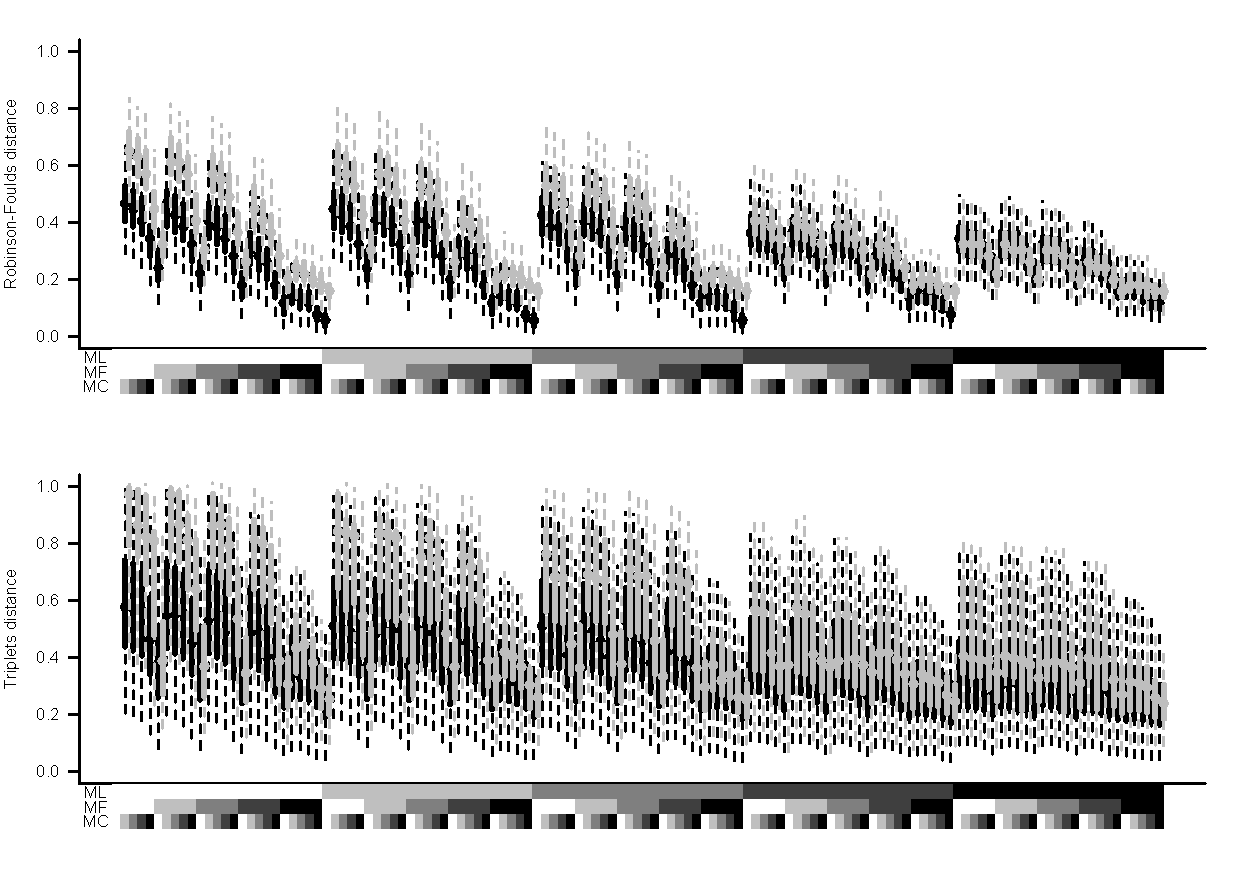
\includegraphics[width=1\textwidth]{SupplementaryMaterial/Supp_Figures/Boot+Baytre-AllParam-RF+Tr.pdf}
\caption{Trend of the effect of missing data on topological recovery on the Bootstraps and the Bayesian posterior trees distributions. The amount of missing data per parameter ($M_{L}$, $M_{F}$ and $M_{C}$) is represented along the x axis. The colour gradient from white to black represents respectively, 0\%, 10\%, 25\%, 50\% and 75\% of missing data. The topological recovery is represented on the y axis, both using Robinson-Foulds distance (upper row) and Triplets distance (lower row). Points represent the modal value of each distribution ; thick solid and thin dashed lines represents respectively the 50\% and 95\% confidence intervals or the distributions. The Bootstraps are represented in black and the Bayesian posterior trees distributions in grey.}
\label{Fig_global_BootTreesets} %Differences between all the parameters and between two methods (Boot vs treesets)
\end{figure}

\begin{figure} 
\centering
    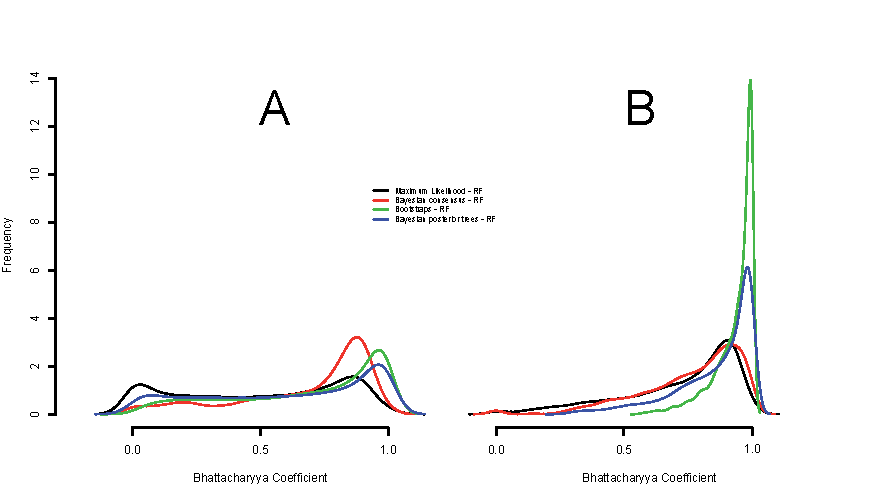
\includegraphics[width=1\textwidth]{SupplementaryMaterial/Supp_Figures/BC-AllMethods-RF+Tr.pdf}
\caption{Distribution of the Pairwise Bhattacharyya Coefficients within each method. A- Distribution of the coefficients when comparing Ronbinson-Foulds distances. B- Distribution of the coefficients when comparing Triplets distances.}
\label{Fig_Bhatt.coeff_distribution} %Differences in overlap within each method
\end{figure}

\begin{figure} 
\centering
    \includegraphics[width=1\textwidth]{SupplementaryMaterial/Supp_Figures/PairwiseComp-ML-RF+Tr.pdf}
\caption{Pairwise Bhattacharyya Coefficients within the Maximum Likelihood trees. The pairwise trees comparisons are represent on both axis. The colour gradient from white to black represents respectively, 0\%, 10\%, 25\%, 50\% and 75\% of missing data for each parameter. The matrix represents the values of pairwise Bhattacharyya Coefficients going from green (1) to red (0). A. Results for the Normalised Robinson-Foulds distance. B. Results with the for Normalised Triplets distance.}
\label{Fig_pairComp-Baytree-RF}
\end{figure} %Pairwise BC for the ML for RF+Tr. (parameters differences)

\begin{figure} 
\centering
    \includegraphics[width=1\textwidth]{SupplementaryMaterial/Supp_Figures/PairwiseComp-Boot-RF+Tr.pdf}
\caption{Pairwise Bhattacharyya Coefficients within the Bootstrap trees. The pairwise trees comparisons are represent on both axis. The colour gradient from white to black represents respectively, 0\%, 10\%, 25\%, 50\% and 75\% of missing data for each parameter. The matrix represents the values of pairwise Bhattacharyya Coefficients going from green (1) to red (0). A. Results for the Normalised Robinson-Foulds distance. B. Results with the for Normalised Triplets distance.}
\label{Fig_pairComp-Baytree-Tr}
\end{figure} %Pairwise BC for the Boot for RF+Tr. (parameters differences)

\begin{figure} 
\centering
    \includegraphics[width=1\textwidth]{SupplementaryMaterial/Supp_Figures/PairwiseComp-Baytre-RF+Tr.pdf}
\caption{Pairwise Bhattacharyya Coefficients within the Bayesian posterior distribution trees. The pairwise trees comparisons are represent on both axis. The colour gradient from white to black represents respectively, 0\%, 10\%, 25\%, 50\% and 75\% of missing data for each parameter. The matrix represents the values of pairwise Bhattacharyya Coefficients going from green (1) to red (0). A. Results for the Normalised Robinson-Foulds distance. B. Results with the for Normalised Triplets distance.}
\label{Fig_pairComp-MLbest-RF}
\end{figure} %Pairwise BC for the Baytre for RF+Tr. (parameters differences)


\begin{table}[ht]
\centering
\begin{tabular}{rrrrrrr}
  \hline
 & Min. & 1st Qu. & Median & Mean & 3rd Qu. & Max. \\ 
  \hline
  Maximum likelihood-RF & 0.06 & 0.26 & 0.40 & 0.41 & 0.50 & 0.95 \\ 
  Maximumlikelihood-Tr & 0.29 & 0.45 & 0.59 & 0.63 & 0.84 & 1.00 \\ 
  Bayesian consensus-RF & 0.69 & 0.71 & 0.72 & 0.76 & 0.79 & 0.96 \\ 
  Bayesian consensus-Tr & -0.28 & -0.11 & 0.17 & 0.19 & 0.37 & 0.98 \\ 
  Bootstraps-RF & 0.06 & 0.18 & 0.27 & 0.26 & 0.34 & 0.46 \\ 
  Bootstraps-Tr & 0.23 & 0.31 & 0.35 & 0.38 & 0.45 & 0.58 \\ 
  Bayesian posterior trees-RF & 0.16 & 0.22 & 0.32 & 0.34 & 0.42 & 0.65 \\ 
  Bayesian posterior trees-Tr & 0.24 & 0.35 & 0.40 & 0.50 & 0.67 & 0.98 \\ 
   \hline
   \hline
\end{tabular}
\end{table}
  \label{Supp_results}

%END
\end{document}